\documentclass{elegantbook}

\definecolor{LightGray}{gray}{0.9}
\newcommand{\CN}{BIOS 7300\\[0.5cm] Survival Data Analysis}
\newcommand{\Ti}{Homework 9}
\newcommand{\Pf}{Dr.\ Tang}
\newcommand{\FN}{Zehao}
\newcommand{\LN}{Wang}
\usepackage[fontsize=14pt]{fontsize}

\usepackage{longtable}

\usepackage{minted}

\usepackage{enumitem}
\renewcommand{\chaptername}{Homework}
\begin{document}
\begin{titlepage}
    \begin{center}    
    
\includegraphics[width=0.6\textwidth]{Tulane.png}\\[1cm]    
    
    \textsc{\Huge \CN}\\[0.5cm]
    \textsc{\large \Pf}\\[1.0cm]
    
    \textsc{\LARGE \Ti}\\[0.5cm]
    \textsc{\large \LN, \FN}\\
    {Master student in Statistics of Math Dept.}
    
    % Author and supervisor
    
    \vfill
    
    % Bottom of the page
    {\Large \emph{\today}}
    
    \end{center}
\end{titlepage}

\thispagestyle{empty}
\tableofcontents
\setcounter{chapter}{8}
\chapter{}

    Freireich et al. (1963) present the following remission times in weeks from a clinical trial in acute leukemia (From Kalbfleisch and Prentice, The Statistical Analysis of Failure Time Data):

    Placebo: 1, 1, 2, 2, 3, 4, 4, 5, 5, 8, 8, 8, 8, 11, 11, 12, 12, 17, 22, 23

    6-MP: 6, 6, 6, 7, 10, 13, 16, 22, 23, 6+, 9+, 10+, 11+, 17+, 19+, 20+, 25+, 32+, 32+, 34+, 35+

\begin{exercise*}[1]
    Use the Placebo group data.
    \begin{enumerate}[(a)]
        \item Examine graphically whether the data should be considered to be a random sample from an exponential distribution.
        \item Fit the data with an exponential distribution.
        \item Estimate the median survival time and its $95\%$ confidence interval based on part (b).
    \end{enumerate}
\end{exercise*}

\begin{solution}
    \begin{minted}[frame=lines,
        framesep=2mm,
        baselinestretch=1.2,
        bgcolor=LightGray,
        fontsize=\footnotesize,
        breaklines=true]{SAS}
PROC IMPORT
    datafile=
    "Y:\Documents\GitHub\MS-Stat-Tulane\Survival_Data_Analysis\HW09\HW9.csv"
    OUT=HW9
    DBMS=csv
    replace;
    GETNAMES=yes;
RUN;

DATA HW9_1;
    SET HW9;
    IF group = 1
    THEN DELETE;
RUN;

PROC LIFETEST DATA=HW9_1 METHOD=km PLOTS=lls;
TIME time*status(1);
RUN;
    \end{minted}
    \begin{enumerate}[(a)]
        \item \begin{figure}[H]
            \centering
            \includegraphics[width=0.8\textwidth]{HW9_1a.png}
        \end{figure}
        The plot is almost a straight line, so it is appropriate to consider the data as a random sample from an exponential distribution.
        \item \begin{minted}[frame=lines,
            framesep=2mm,
            baselinestretch=1.2,
            bgcolor=LightGray,
            fontsize=\footnotesize,
            breaklines=true]{SAS}
PROC LIFEREG DATA=HW9_1;
MODEL time*status(1)=/d=exponential;
OUTPUT out=a p=median std=se;
PROBPLOT/nodata;
INSET;
RUN;
        \end{minted}
        \begin{figure}[H]
            \centering
            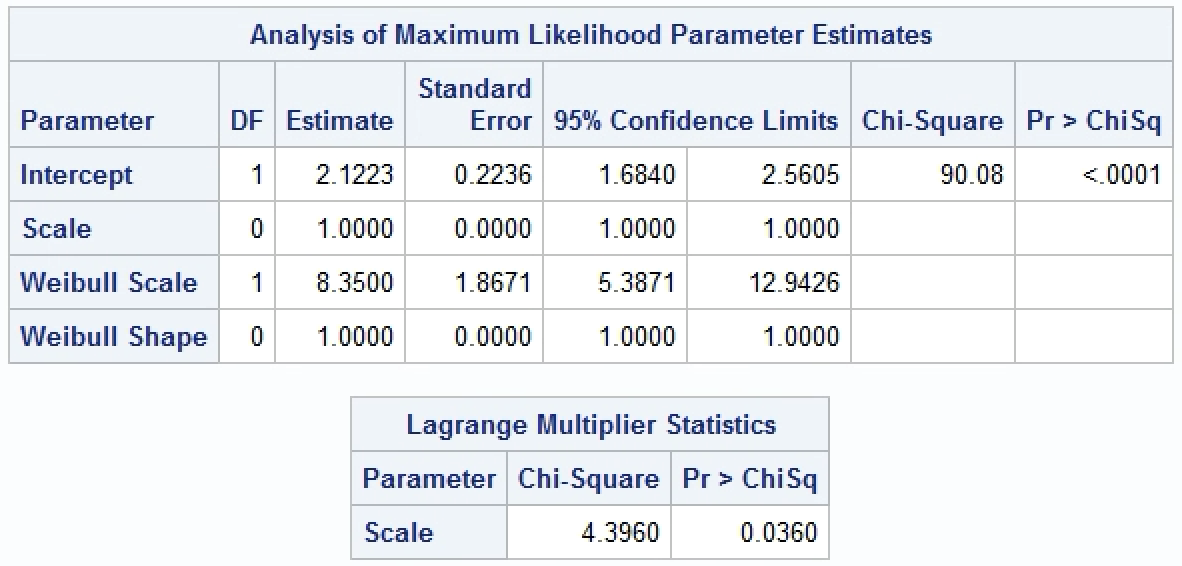
\includegraphics[width=0.8\textwidth]{HW9_1b.png}
        \end{figure}
        \item \begin{minted}[frame=lines,
            framesep=2mm,
            baselinestretch=1.2,
            bgcolor=LightGray,
            fontsize=\footnotesize,
            breaklines=true]{SAS}
DATA a;
SET a;
upper=median + 1.96 * se;
lower=median - 1.96 * se;
RUN;

PROC PRINT DATA=a;
RUN;
        \end{minted}
        \begin{figure}[H]
            \centering
            \includegraphics[width=0.8\textwidth]{HW9_1c.png}
        \end{figure}
        Median survival time is $5.7877$, and its $95\%$ confidence interval is $[3.251, 8.324]$.
    \end{enumerate}
\end{solution}

\begin{exercise*}[2]
    Use the Placebo group data.
    \begin{enumerate}[(a)]
        \item Examine graphically whether the data might be considered to be a random sample from a Weibull distribution.
        \item Fit the data with a Weibull distribution, and estimate the median survival time and its $95\%$ confidence interval.
        \item Based on the fitting of the Weibull distribution, does the data follow an exponential distribution?
    \end{enumerate}
\end{exercise*}

\begin{solution}
    \begin{enumerate}[(a)]
        \item \begin{minted}[frame=lines,
            framesep=2mm,
            baselinestretch=1.2,
            bgcolor=LightGray,
            fontsize=\footnotesize,
            breaklines=true]{SAS}
PROC UNIVARIATE DATA=HW9_1;
VAR time;
HISTOGRAM time/weibull;
RUN;
        \end{minted}
        \begin{figure}[H]
            \centering
            \includegraphics[width=0.8\textwidth]{HW9_2a.png}
            \includegraphics[width=0.5\textwidth]{HW9_2a1.png}
        \end{figure}
        From the histogram, we can see that the data is consistent with a Weibull distribution. And the p-value of the goodness-of-fit test $>0.05$, so we can conclude that the data is a random sample from a Weibull distribution. 
        \item \begin{minted}[frame=lines,
            framesep=2mm,
            baselinestretch=1.2,
            bgcolor=LightGray,
            fontsize=\footnotesize,
            breaklines=true]{SAS}
PROC LIFEREG DATA=HW9_1;
MODEL time*status(1)=/d=weibull;
OUTPUT out=a p=median std=se;
PROBPLOT/nodata;
INSET;
RUN;

DATA a;
SET a;
upper=median + 1.96 * se;
lower=median - 1.96 * se;
RUN;

PROC PRINT DATA=a;
RUN;
        \end{minted}
        \begin{figure}[H]
            \centering
            \includegraphics[width=0.6\textwidth]{HW9_2b.png}
            \includegraphics[width=0.6\textwidth]{HW9_2b1.png}
        \end{figure}
        Median survival time is $6.9238$, and its $95\%$ confidence interval is $[4.249, 9.598]$.
        \item \begin{figure}[H]
            \centering
            \includegraphics[width=0.8\textwidth]{HW9_2c.png}
        \end{figure}
        Shape parameter is $1.338$, which is close to $1$. So the data is more consistent with an exponential distribution. 
    \end{enumerate}
\end{solution}

\begin{exercise*}[3]
    Apply a Weibull proportional hazards model to the whole data.
    \begin{enumerate}[(a)]
        \item Test for adequacy of an exponential model relative to the Weibull model.
        \item Test the hypothesis of equality of remission times in the two groups using Weibull model.
        \item Estimate the hazards ratio at the same time points between the two groups based on the Weibull model.
        \item Estimate the ratio of the 80 percentile survival times of the two groups based on the Weibull model.
    \end{enumerate}
\end{exercise*}

\begin{solution}
    \begin{enumerate}[(a)]
        \item \begin{minted}[frame=lines,
            framesep=2mm,
            baselinestretch=1.2,
            bgcolor=LightGray,
            fontsize=\footnotesize,
            breaklines=true]{SAS}
PROC LIFETEST DATA=HW9 METHOD=km PLOTS=lls;
TIME time*status(1);
STRATA group;
RUN;
        \end{minted}
        \begin{figure}[H]
            \centering
            \includegraphics[width=0.65\textwidth]{HW9_3a.png}
        \end{figure}
        From the log-log survival plot, we can see the line for two groups are almost parallel, and are straight lines. So, the exponential model is better than the Weibull model.
    \item \begin{minted}[frame=lines,
        framesep=2mm,
        baselinestretch=1.2,
        bgcolor=LightGray,
        fontsize=\footnotesize,
        breaklines=true]{SAS}
PROC LIFEREG DATA=HW9;
CLASS group;
MODEL time*status(1)=group/d=weibull;
OUTPUT out=a p=median std=se;
PROBPLOT;
RUN;
        \end{minted}
        \begin{figure}[H]
            \centering
            \includegraphics[width=0.65\textwidth]{HW9_3b.png}
        \end{figure}
        Compared to 6-MP group, we can see that the estimate for Placebo group is $-1.3131$, and the p-value is $<0.0001$. So, the Placebo group has a lower hazards than 6-MP group. 
        \item \[HR(Placebo\ V.S.\ 6-MP)=\exp(-1.3131)=0.26898. \]
        \item \begin{minted}[frame=lines,
            framesep=2mm,
            baselinestretch=1.2,
            bgcolor=LightGray,
            fontsize=\footnotesize,
            breaklines=true]{SAS}
PROC LIFEREG DATA=HW9;
CLASS group;
MODEL time*status(1)=group/d=weibull;
OUTPUT out=a p=p80 q=0.8;
PROBPLOT;
RUN;

PROC PRINT DATA=a;
RUN;
            \end{minted}
            \begin{figure}[H]
                \centering
                \includegraphics[width=0.35\textwidth]{HW9_3d.png}
            \end{figure}
            So, the ratio of the 80 percentile survival times of the two groups is $12.995/48.3117=0.26899$. 
    \end{enumerate}
\end{solution}
\end{document}



